\documentclass{article}
\usepackage[utf8x]{inputenc}
\usepackage{ucs}
\usepackage{amsmath} 
\usepackage{amsfonts}
\usepackage{marvosym}
\usepackage{wasysym}
\usepackage{upgreek}
\usepackage[english,russian]{babel}
\usepackage{graphicx}
\usepackage{float}
\usepackage{textcomp}
\usepackage{hyperref}
\usepackage{geometry}
  \geometry{left=2cm}
  \geometry{right=1.5cm}
  \geometry{top=1cm}
  \geometry{bottom=2cm}
\usepackage{tikz}
\usepackage{ccaption}
\usepackage{multicol}

\usepackage{listings}
%\setlength{\columnsep}{1.5cm}
%\setlength{\columnseprule}{0.2pt}

\usepackage{colortbl,graphicx,tikz}
\definecolor{X}{rgb}{.5,.5,.5}

\title{ДЗ. Работа с изображениями в формате \texttt{.ppm}}
\date{}
\begin{document}
\pagenumbering{gobble}

\lstset{
  language=C++,                % choose the language of the code
  basicstyle=\linespread{1.1}\ttfamily,
  columns=fixed,
  fontadjust=true,
  basewidth=0.5em,
  keywordstyle=\color{blue}\bfseries,
  commentstyle=\color{gray},
  stringstyle=\ttfamily\color{orange!50!black},
  showstringspaces=false,
  %numbers=false,                   % where to put the line-numbers
  numbersep=5pt,
  numberstyle=\tiny\color{black},
  numberfirstline=true,
  stepnumber=1,                   % the step between two line-numbers.        
  numbersep=10pt,                  % how far the line-numbers are from the code
  backgroundcolor=\color{white},  % choose the background color. You must add \usepackage{color}
  showstringspaces=false,         % underline spaces within strings
  captionpos=b,                   % sets the caption-position to bottom
  breaklines=true,                % sets automatic line breaking
  breakatwhitespace=true,         % sets if automatic breaks should only happen at whitespace
  xleftmargin=.2in,
  extendedchars=\true,
  keepspaces = true,
}
\lstset{literate=%
   *{0}{{{\color{red!20!violet}0}}}1
    {1}{{{\color{red!20!violet}1}}}1
    {2}{{{\color{red!20!violet}2}}}1
    {3}{{{\color{red!20!violet}3}}}1
    {4}{{{\color{red!20!violet}4}}}1
    {5}{{{\color{red!20!violet}5}}}1
    {6}{{{\color{red!20!violet}6}}}1
    {7}{{{\color{red!20!violet}7}}}1
    {8}{{{\color{red!20!violet}8}}}1
    {9}{{{\color{red!20!violet}9}}}1
}


\section*{Домашнее задание \#1: Ссылки и перегрузка операторов}
\subsection*{Пространство имён:}
\begin{itemize}
\item Создайте пространство имён по имени \texttt{myspace}. В этом пространстве имён создайте функцию \\
 \texttt{void print\_n\_times(char str[], int n = 10)}, которая будет печатать строку \texttt{str} \texttt{n} раз. Для печати используйте \texttt{std::cout} из библиотеки \texttt{iostream}. Вызовите эту функцию из \texttt{main}.
\end{itemize}

\subsection*{Ссылки:}
\begin{itemize}
\item Напишите функцию \texttt{cube}, которая будет принимать одно число типа \texttt{int} и возводить его в куб. Используёте ссылки.
\item Напишите функцию \texttt{void count\_letters(char str[], int\& n\_letters, int\& n\_digits, int\& n\_other)}, которая будет принимать на вход строку \texttt{str} и подсчитывать число букв и цифр в этой строке. Количество букв нужно записать в переменную \texttt{n\_letters}, количество цифр -- в переменную \texttt{n\_digits}, а количество остальных символов -- в переменную \texttt{n\_other}. Вызвать эту функцию из функции \texttt{main} и проверить её работу.
\end{itemize}

\subsection*{Перегрузка операций:}
В файлах \texttt{code/complex.h} и \texttt{code/complex.cpp} лежит реализация комплексного числа с перегруженными операторами. Используёте его в качестве примера для решения задач этого раздела:
\begin{itemize}
\item Создайте структуру \texttt{Vector3f} - вектор в трёхмерном пространстве с полями \texttt{x, y, z} типа \texttt{float} в качестве координат. Перегрузите следующие операторы для работы с вектором. Для передачи вектора в функции используте ссылки и, там где возможно, модификатор \texttt{const}.
	\begin{itemize}
	\item Сложение векторов (\texttt{+})
	\item Вычитание (\texttt{-})
	\item Умножение вектора на число типа \texttt{float} (число \texttt{*} вектор и вектор \texttt{*} число)
	\item Деление вектора на число типа \texttt{float} (вектор \texttt{/} число)
	\item Скалярное произведение (\texttt{*})
	\item Векторное произведение (\texttt{\^})
	\item Унарный \texttt{-}
	\item Унарный \texttt{+}
	\item Проверка на равенство \texttt{==}  (должна возвращать тип \texttt{bool})
	\item Проверка на неравенство \texttt{!=}  (должна возвращать тип \texttt{bool})
	\item Операторы \texttt{+=} и \texttt{-=}  (вектор \texttt{+=} вектор)
	\item Операторы \texttt{*=} и \texttt{/=}  (вектор \texttt{*=} число)
	\item Оператор вывода  \texttt{ostream >{}>} вектор. Выводите вектор в виде \texttt{(x, y, z)}.
	\item Оператор ввода  \texttt{istream <{}<} вектор
	\item Функция \texttt{float squared\_norm(const Vector3f\& a)}, которая вычисляет квадрат нормы вектора.
	\item Функция \texttt{float norm(const Vector3f\& a)}, которая вычисляет норму вектора.
	\item Функция \texttt{void normalize(Vector3f\& a)}, которая нормализует вектор \texttt{a}.
	\end{itemize}
\item Поместите весь ваш код в отдельный файл \texttt{vector3f.h} и подключите к файлу \texttt{main.cpp}.
\item Протестируйте ваши функции:
\begin{lstlisting}
#include <iostream>
#include "vector3f.h"

using namespace std;


int main() {
	Vector3f a = {1.0, 2.0, -2.0};
	Vector3f b = {4.0, -1.0, 3.0};
	cout << "a = " << a << endl << "b = " << b << endl;
	cout << "a + b = " << a + b << endl;
	cout << "-a = " << -a << endl;
	cout << "Scalar product of a and b = " << a * b << endl;
	cout << "Cross product of a and b = " << a ^ b << endl;
	a /= 5;
	cout << "a after a /= 5;"  << a << endl
	normalize(b);
	cout << "Normalized b:"  << b << endl
}
\end{lstlisting}
\item Аналогично опишите типы \texttt{Vector3d} (3 координаты типа \texttt{double}), \texttt{Vector3i} (3 координаты типа \texttt{int}), \texttt{Vector2f}, \texttt{Vector2d}, \texttt{Vector2i}, \texttt{Vector4f} (может понадобится когда-нибудь). Каждый новый тип нужно описать в отдельном файле. Для векторов размерности 2 и 4 можно не писать векторное произведение.

\end{itemize}
\subsection*{Задача об убегающей точке}
\begin{itemize}
\item Предположим, что у нас есть комплексная функция $f(z) = z^2$. Выберем некоторое комплексное число $z_0$ и будем проводить следующие итерации: 
\begin{equation}
\label{fractalseq}
z_1 = f(z_0)\quad z_2 = f(z_1)\quad ...\quad z_{k+1} = f(z_k)\quad ...
\end{equation}
В зависимости от выбора точки $z_0$ эта последовательность либо разойдётся, либо останется в некоторой ограниченной области. Будем называть точку $z_0$ убегающей, если $z_k \rightarrow \infty$ при $k \rightarrow \infty$. Найдите область неубегания для функции $z^2$, т.е. множество всех начальных значений $z_0$, при которых последовательность (\ref{fractalseq}) остаётся ограниченной (это можно сделать в уме). \\

\item \textbf{Julia:} Для функции $f(z) = z^2$ эта область тривиальна, но всё становится сложней для функции вида $f(z) = z^2 + c$, где $c$ -- некоторое комплексное число. Численно найдите область неубегания для функций такого вида. Для этого создайте изображение размера 800x800, покрывающую область \texttt{[-2:2]x[-2:2]} на комплексной плоскости. Для каждой точки этой плоскости проведите $N \approx 20$ итераций и, в зависимости от результата, окрасьте пиксель в соответствующий цвет (цвет можно подобрать самим, он должен быть пропорционален значению $z_N$ - меняться от яркого если $z_N$ мало и до черного если $z_N$ большое). Используйте класс Complex и перегруженные операторы. Пример работы с изображениями в формате \texttt{ppm} можно посмотреть в фале \texttt{complex\_image.cpp}. Программа должна создавать файл \texttt{julia.ppm}.

\begin{center}
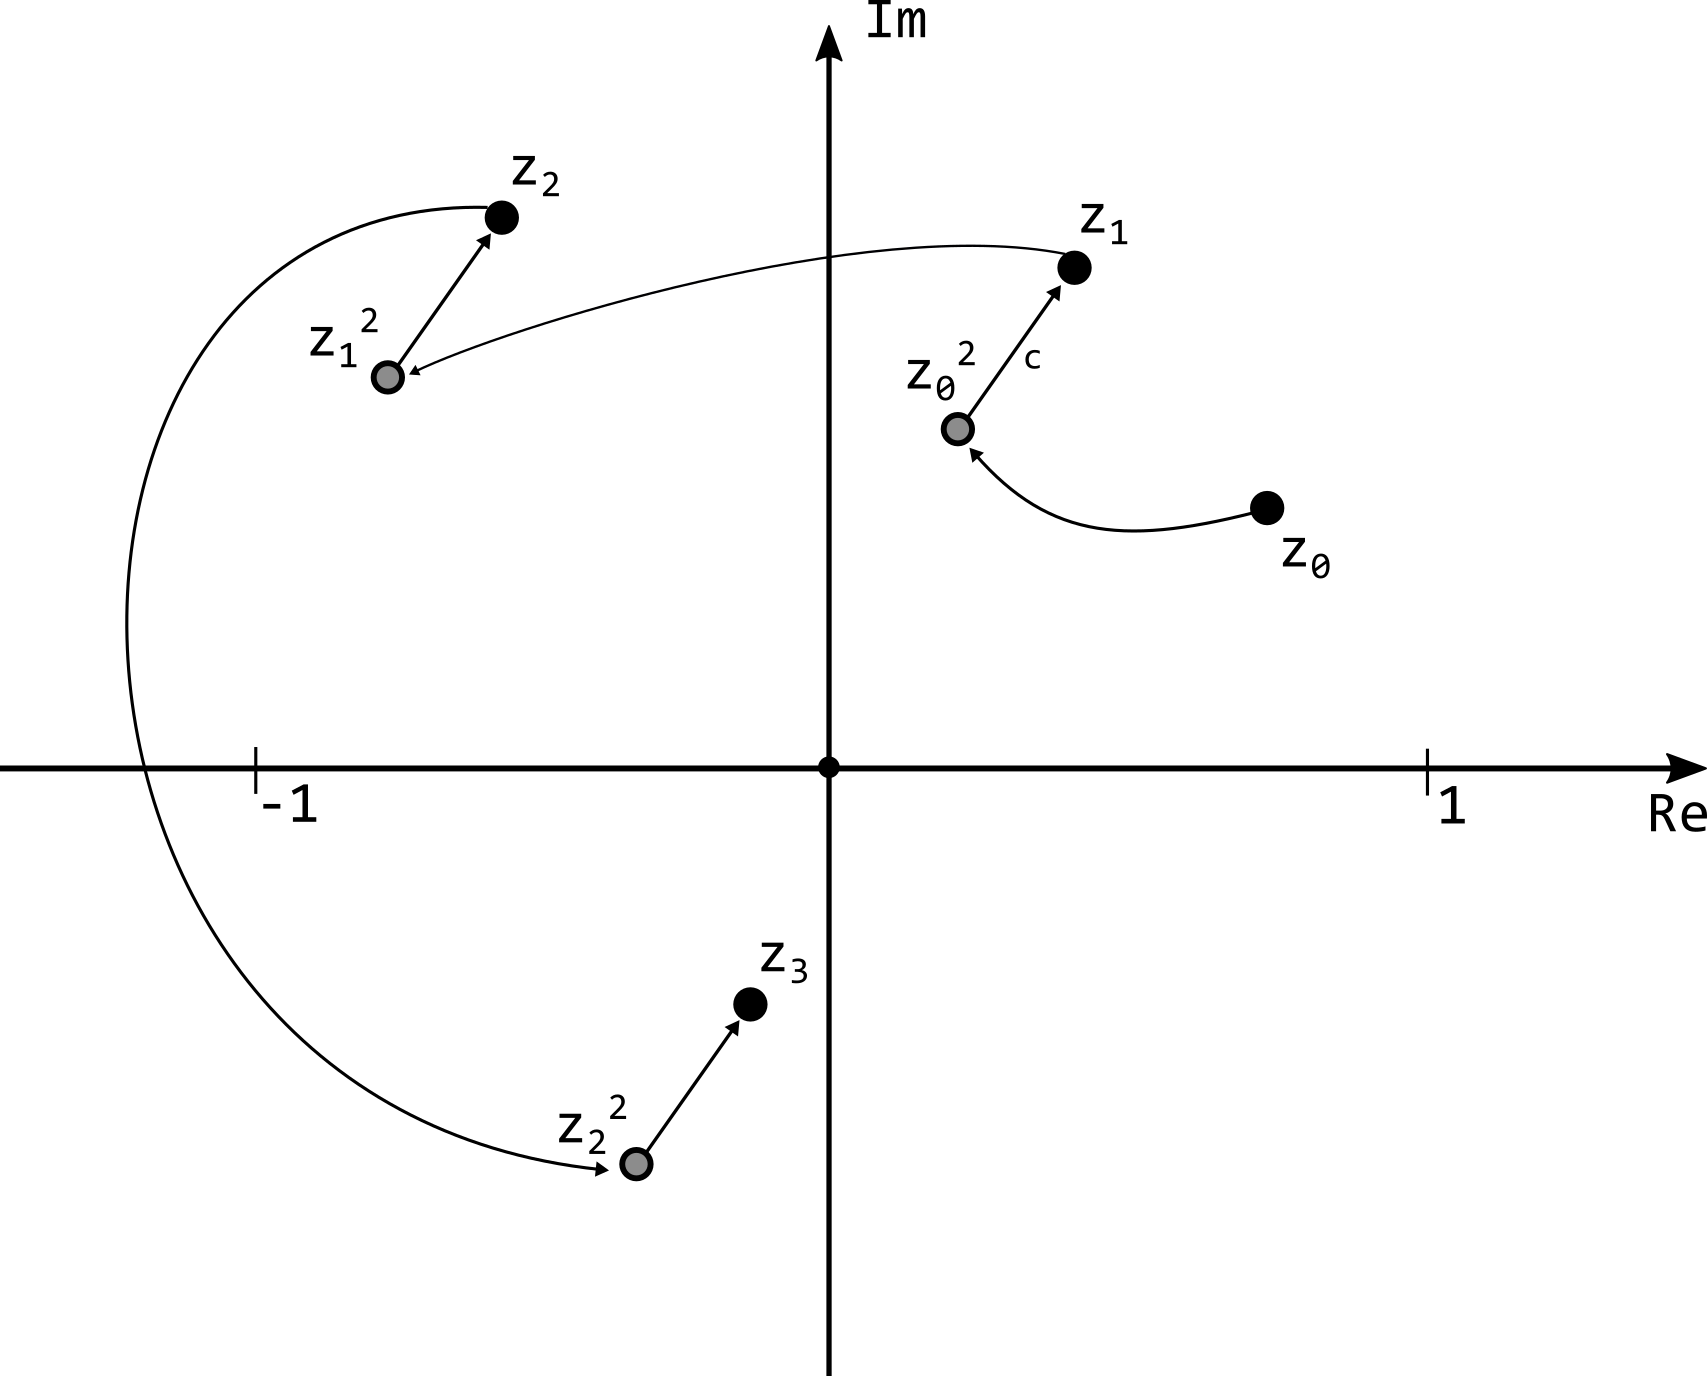
\includegraphics[scale=0.7]{../images/complexplane.png}
\end{center}

\item Нарисуте изображение для $c = -0.4 + 0.6i$;\quad $c = -0.70 - 0.38i$;\quad $c = -0.80 + 0.16i$\quad  и\quad $c = 0.280 + 0.011i$.
\item Добавьте параметры командной строки: 2 вещественных числа, соответствующие комплексному числу $c$, и целое число итераций $N$. 
\item \textbf{Mandelbrot:} Зафиксируем теперь $z_0 = 0$ и будем менять $c$. Численно найдите все параметры $c$, для которых точка $z_0$ не является убегающей. Для этого создайте изображение размера 800x800, покрывающую область \texttt{[-2:2]x[-2:2]} возможных значений $c$ на комплексной плоскости. Программа должна создавать файл \texttt{mandelbrot.ppm}.

\item \textbf{Анимация:} Программа \texttt{complex\_movie.cpp} создаёт множество изображений и сохраняет их в папку \texttt{animation} (если у вас нет такой папки -- создайте её). Эти изображения представляют собой отдельные кадры будущей анимации. Чтобы их объединить в одно видео можно использовать программу ffmpeg (Нужно скачать тут: \href{https://www.ffmpeg.org/}{www.ffmpeg.org} и изменить переменную среды \texttt{PATH} в настройках Windows или Linux). После этого можно будет объединить все изображения в одно видео такой командой:
\begin{verbatim}
ffmpeg -r 60 -i animation/complex_%03d.ppm complex_movie.mp4
\end{verbatim}
Создайте анимацию из изображений множеств Julia при $c$ линейно меняющемся от $(-1.5 - 0.5i)$ до $i$.
\end{itemize}
\end{document}